\documentclass[tikz]{standalone}
\usepackage{tikz}
\usetikzlibrary{calc,arrows,decorations.pathmorphing, decorations.pathreplacing,backgrounds,positioning,fit,petri,shapes.misc,graphs}
\begin{document}
\tikzset{
    node distance=5mm,
    terminal/.style={
                    % The shape:
                    rounded rectangle,
                    minimum size=6mm,
                    % The rest
                    very thick,draw=black!50,
                    top color=white,bottom color=black!20,
                    font=\ttfamily},
    nonterminal/.style={
                        % The shape:
                        rectangle,
                        % The size:
                        minimum size=6mm,
                        % The border:
                        very thick,
                        draw=red!50!black!50, % 50% red and 50% black,
                        % and that mixed with 50% white
                        % The filling:
                        top color=white, % a shading that is white at the top...
                        bottom color=red!50!black!20, % and something else at the bottom
                        % Font
                        font=\itshape
                        }}
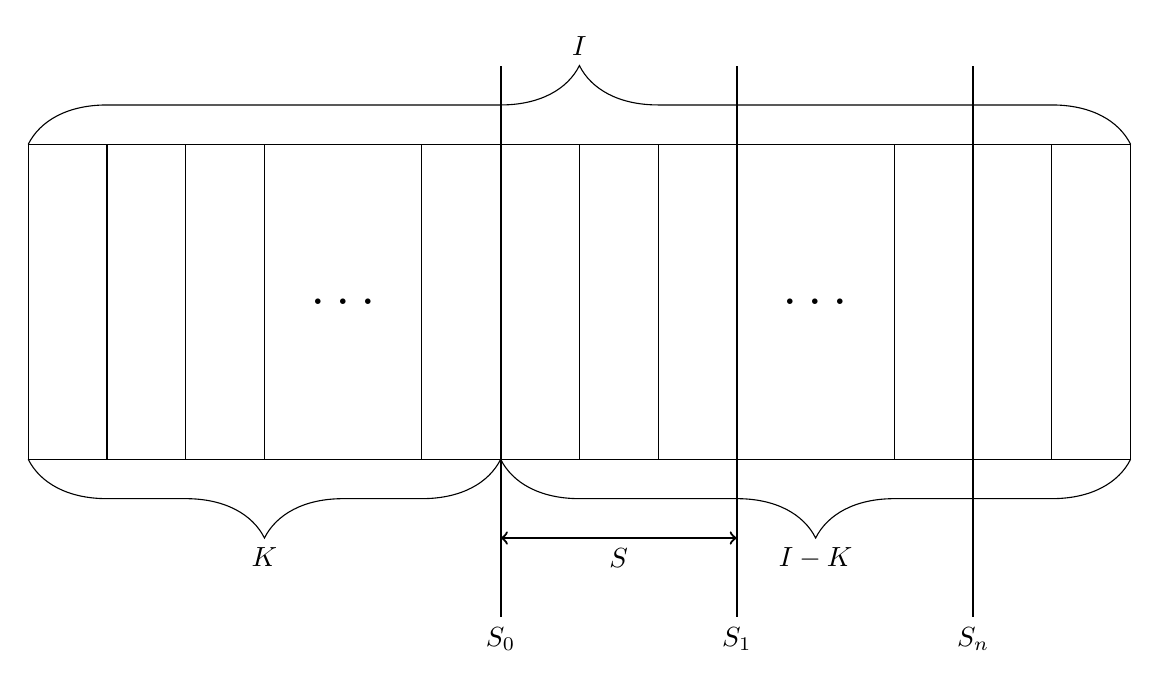
\begin{tikzpicture}
    % pos能指定node在路径纵向上的位置,按比例
    [down_brace_label/.style={pos=0.5, yshift=-1cm, anchor=north, auto, sloped, swap},
    up_brace_label/.style={pos=0.5, yshift=1cm, anchor=south, auto, sloped}]
    % 绘制网格
    \draw[xstep=1cm, ystep=4cm] (0, 0) grid (3, 4);
    \draw (3, 0) rectangle (5, 4);
    \draw[xstep=1cm, ystep=4cm] (5, 0) grid (9, 4);
    \draw (9, 0) rectangle (11, 4);
    \draw[xstep=1cm, ystep=4cm] (11, 0) grid (14, 4);
    % 绘制括号与标签
    \draw [decorate, decoration={brace, amplitude=1cm}] 
    (0, 4) -- node[up_brace_label]{$I$} (14, 4);
    \draw [decorate, decoration={brace, mirror, amplitude=1cm}] 
    (0, 0) -- node[down_brace_label]{$K$} (6, 0);
    \draw [decorate, decoration={brace, mirror, amplitude=1cm}] 
    (6, 0) -- node[down_brace_label]{$I-K$} (14, 0);
    \node at (4, 2) {\huge $\dots$};
    \node at (10, 2) {\huge $\dots$};
    % 绘制竖线
    \draw[thick] (6, -2) node[anchor=north]{$S_0$} -- (6, 5);
    \draw[thick] (9, -2) node[anchor=north]{$S_1$} -- (9, 5);
    \draw[thick] (12, -2) node[anchor=north]{$S_n$} -- (12, 5);
    % 绘制S宽度线
    \draw[<->, thick] (6, -1) -- node[anchor=north, sloped]{$S$} (9, -1);
\end{tikzpicture}

\end{document}